\documentclass[11pt,a4paper]{article}
\usepackage[utf8]{inputenc}
\usepackage[T1]{fontenc}
\usepackage{lmodern}
\usepackage[margin=2.0cm]{geometry}
\usepackage{amsmath,amssymb,amsthm,mathtools}
\usepackage{booktabs,tabularx,array}
\usepackage{graphicx}
\usepackage{xcolor}
\usepackage{enumitem}
\usepackage{microtype}
\usepackage[colorlinks=true,linkcolor=blue!55!black,citecolor=blue!55!black,urlcolor=blue!55!black]{hyperref}

\renewcommand{\abstractname}{Kivonat}
\renewcommand{\contentsname}{Tartalomjegyzék}
\renewcommand{\figurename}{Ábra}
\renewcommand{\tablename}{Táblázat}
\renewcommand{\refname}{Irodalomjegyzék}
\renewcommand{\proofname}{Bizonyítás}

\setlength{\emergencystretch}{3em}
\newtheorem{theorem}{Tétel}[section]
\newtheorem{proposition}[theorem]{Állítás}
\newtheorem*{remark}{Megjegyzés}

\title{\textbf{A diszkrét tetraéderes Clifford-pregeometriától a\\
négydimenziós Lorentz-invariáns kontinuumig}\\[0.35em]
\large Mindenhurkos \texorpdfstring{$\mathrm{Pin}(W(F_4))$}{Pin(W(F4))} izotrópia a 24-cellás rácson, Osterwalder--Schrader rekonstrukció\\
és a kitüntetett-rendszerű gravitáció Stueckelberg--Lorenz lezárása}

\author{\textbf{Olcsák József}\\
\small Független kutató $\cdot$ ORCID: \href{https://orcid.org/0009-0003-7311-6522}{0009-0003-7311-6522}\\
\small E-mail: \href{mailto:jolcsak@gmail.com}{jolcsak@gmail.com}}
\date{2026.\ november 20.}

\begin{document}
\maketitle

\begin{abstract}
\raggedright
\noindent Minden diszkrét pregeometriai kvantumgravitációs és nagy egyesítési elmélet két szigorú ultraibolya--infravörös akadállyal szembesül: (1) a gamma-kitörések (GRB) futási ideje, a kozmológiai polarimetria, az ultra-nagyenergiás kozmikus sugárzás (UHECR) és a Collins--Perez--Sudarsky--Urrutia--Vucetich (CPSUV) sugárzási perkolációs tétel $12$--$19$ nagyságrenddel kizárja az általános Planck-skálás diszkretizációkat; (2) a módosított newtoni dinamika infravörös egység-időszerű direktor-kiterjesztései (\texttt{COV-DIR+QUMOND}) vagy $\mathcal{O}(1)$ paraméterezett poszt-newtoni (PPN) kitüntetett-rendszerű anomáliákat ($\alpha_1^{\mathrm{PPN}}, \alpha_2^{\mathrm{PPN}}$), vagy inhomogén Sturm--Liouville kinetikus szellemeket kockáztatnak. Jelen tanulmányban mindkét problémát új szabad paraméter nélkül ($k_{\mathrm{dark}} = 0$) oldjuk meg a diszkrét tetraéderes ($K_4$, $N = 4$) szimpliciális-Clifford keretrendszerben. Először egzakt algebrai azonosságot igazolunk az $|\nu|=1$ plakett-területkvantum ($\ell_*^2 = 24\pi\ell_P^2$) és a nagy egyesítési / Starobinsky UV-levágás között: $\ell_*^{-1} \equiv M_{\mathrm{Pl}}/\sqrt{3} \equiv M_* = 1.4060\times 10^{18}\;\mathrm{GeV}$. Másodszor No-Go tétellel kizárjuk a merev háromdimenziós $+K_4$ és párosított gyémánt $(+K_4\oplus -K_4)$ kristályrácsokat a LHAASO GRB~221009A ($E_{\mathrm{QG},1} \ge 10\,E_{\mathrm{Pl}}$), a GRB vákuum-kettőstörés és a CPSUV egyhurkos perkoláció alapján. Harmadszor bebizonyítjuk, hogy a $T \cong A_4$ tetraédercsoport spin-kétszeres fedése -- a $2T \subset \mathrm{Spin}(3) \cong S^3$ bináris tetraédercsoport ($|2T| = 24 = 4!$) -- kanonikusan a Hurwitz-féle 24-cellás $\Lambda_{F_4} \cong \Lambda_{D_4}$ Bravais-rácsként ágyazódik be, amelynek $1152$ elemű $W(F_4)$ pontcsoportja indexszimmetria-feltevés nélkül teljesíti az $\mathrm{Inv}_{W(F_4)}((\mathbb{R}^4)^{\otimes r}) \equiv \mathrm{Inv}_{O(4)}((\mathbb{R}^4)^{\otimes r})$ tenzorgyűrű-egyenértékűséget minden $r \in \{1,2,3,4,5\}$ rangra, a $32$ egyenlő oldalú háromszögű Wilson-plakett és a Neuberger-féle Overlap-operátor $\mathrm{Pin}(W(F_4))$ kovarianciája ($1.56\times 10^{-15}$) pedig minden perturbatív hurokrendben azonosan kinullázza az összes $d \le 7$ ($c_{\mu\nu}$, mind a $19$ $k_F$, $n=1,2,3$) Lorentz-sértő operátort; a vezető $d=8$ ($n=4$) csoportsebesség-eltolódás $|\delta v_g/c| = \frac{5}{2}(E/M_*)^4 = 6.72\times 10^{-56}$ ($\Delta t = 6.02\times 10^{-39}\;\mathrm{s}$) a LHAASO $18\;\mathrm{TeV}$-es fotonjainál. Negyedszer igazoljuk az egy-időszeletes bozonikus/mérték Osterwalder--Schrader pozitivitást, mind a $39$ Brillouin-zónabeli fermion-duplikátum kiemelését, a Starobinsky $R + R^2/(6 M_{\mathrm{inf}}^2)$ hatás egzakt Hawking--Luttrell euklideszi diagonalizációját az $|\nu|=1$ kauzális szeleteléssel együtt, valamint a $d_S(\sigma) = 4 + \ell_*^2/(2\sigma) \to 4$ spektrálisdimenzió-futást. Végül a kanonikus Bumblebee direktor-skálát ($V_\mu = f_{\mathrm{dir}} A_\mu$) a Starobinsky-skalaron tömegéhez zárva ($f_{\mathrm{dir}} \equiv M_{\mathrm{inf}} = 3.1959\times 10^{13}\;\mathrm{GeV}$, $c_{\mathrm{acc}} = (M_{\mathrm{inf}}/M_{\mathrm{Pl}})^2 = 1.722\times 10^{-10}$, $c_2 = c_{\mathrm{acc}}/(1 - 2 c_{\mathrm{acc}})$) egyszerre kapunk $c_T = c_V = c_S \equiv 1$-et (azonosan zérus Cserenkov-veszteséget), $\alpha_2^{\mathrm{PPN}} \equiv 0$-t, $\alpha_1^{\mathrm{PPN}} = -6.89\times 10^{-10}$-et és szigorúan pozitív $K_{\alpha\alpha}^{\mathrm{nonpert}} > 0$ Sturm--Liouville sajátértéket a Földtől és a Naptól a SPARC galaxisokon át az X-COP galaxishalmazokig.
\end{abstract}

\tableofcontents
\vspace{0.4em}
\hrule
\vspace{0.8em}

% =============================================================================
\section{Bevezetés és az egzakt plakett--egyesítési skálaazonosság}
\label{sec:intro}
% =============================================================================

A diszkrét kvantumgravitációs mikroszerkezet és a makroszkopikus négydimenziós (4D) lokális Lorentz-invariancia ($\mathrm{SO}^+(1,3)$) összeegyeztetése az elméleti fizika egyik legszigorúbb konzisztenciakapuja \cite{Liberati2013,KosteleckyMewes2002,Addazi2022}. A LHAASO obszervatórium GRB~221009A-ból ($z = 0.151$) érkező $18\;\mathrm{TeV}$-es fotonjai a lineáris ($n=1$, $d=5$) Lorentz-sértést (LIV) az $E_{\mathrm{QG},1} \ge 10.0\,E_{\mathrm{Pl}} \simeq 1.22\times 10^{20}\;\mathrm{GeV}$ tartományba szorítják \cite{LHAASO2024LIV}, a kozmológiai polarimetria $|\xi_{\mathrm{biref}}| \lesssim 10^{-16}$-ra korlátozza a vákuum-kettőstörést, az $E \simeq 10^{20}\;\mathrm{eV}$-os UHECR kozmikus részecskék pedig kizárják a szubluminális gravitációs Cserenkov-sugárzást ($|\delta c| \lesssim 10^{-22}$ \cite{ElliottMooreStoica2005}). Emellett a CPSUV--Polchinski-tétel \cite{CPSUV2004,Polchinski2012} kimondja, hogy bármely, az $O(4)$ szimmetriát $O(3)$-ra sértő UV-levágás a Standard Modell 1-hurkos önenergiáin keresztül elnyomatlan \emph{4-dimenziós} sebességhasadást ($|\Delta c_{ij}/c| \sim g^2/(16\pi^2) \sim 10^{-3}$) generál.

Először rögzítjük az egzakt algebrai hidat az $|\nu|=1$ tetraéderes plakett-területkvantum \cite{Olcsak2026JMP} és a $\mathrm{Spin}(10)$ / Starobinsky UV-egyesítési skála \cite{Olcsak2026Paper24,Olcsak2026Paper25,Olcsak2026Paper26} között:
\begin{proposition}[Egzakt plakett--egyesítési skálaazonosság]
\label{prop:scale-identity}
Az $\ell_P^2 \equiv \hbar G/c^3 = (8\pi M_{\mathrm{Pl}}^2)^{-1}$ Planck-területtel ($M_{\mathrm{Pl}} = 2.435323\times 10^{18}\;\mathrm{GeV}$) a minimális $K_4$ 3-szimplex ($N = 4$) $|\nu|=1$ plakett-területkvantuma, $\ell_*^2 = N!\,\pi\,\ell_P^2 = 24\pi\,\ell_P^2$, azonosan kielégíti az alábbi összefüggést:
\begin{equation}
\ell_*^2 = \frac{24\pi}{8\pi M_{\mathrm{Pl}}^2} = \frac{3}{M_{\mathrm{Pl}}^2}
\quad\Longleftrightarrow\quad
\ell_*^{-1} \equiv \frac{M_{\mathrm{Pl}}}{\sqrt{3}} \equiv M_* = 1.406034\times 10^{18}\;\mathrm{GeV}.
\label{eq:scale-id-hu}
\end{equation}
\end{proposition}

% =============================================================================
\section{No-Go tétel a merev 3D \texorpdfstring{$+K_4$}{+K4} és \texorpdfstring{$3+1\mathrm{D}$}{3+1D} kristályrácsok ellen}
\label{sec:nogo}
% =============================================================================

\begin{theorem}[Merev 3D $+K_4$ és $3+1\mathrm{D}$ kristály No-Go]
\label{thm:3d-nogo}
Az $M_* = \ell_*^{-1} = 1.4060\times 10^{18}\;\mathrm{GeV}$ ($= 0.11516\,E_{\mathrm{Pl}}$) rögzített plakett-skálán mind az egyorientációjú 3D $+K_4$ térrács, mind a párosított gyémánt $(+K_4\oplus -K_4)$ kristály $3+1\mathrm{D}$ időszeleteléssel kísérletileg kizárt.
\end{theorem}

\begin{proof}
A szabályos 3D tetraéder $\mathbf{n}_i \in S^2 \subset \mathbb{R}^3$ ($i=1,\dots,4$) csúcsvektoraira $T^{(m)}(\mathbf{k}) = \sum_{i=1}^4(\mathbf{n}_i\cdot\mathbf{k})^m$ kifejtése $T^{(1)} = 0$, $T^{(2)}(\mathbf{k}) = \frac{4}{3}|\mathbf{k}|^2$, de $T^{(3)}(\mathbf{k}) = \frac{8}{\sqrt{3}}k_x k_y k_z \neq 0$ és $T^{(4)}_{xxxx} - 3T^{(4)}_{xxyy} = -\frac{8}{9} \neq 0$ momentumokat ad (\path{verify_paper27_continuum_lorentz_closure.py}). Az egyorientációjú $+K_4$-ben a térbeli inverzió hiánya miatt fellépő $T^{(3)} \neq 0$ tag paritássértő $d=5$ ($n=1$) lineáris diszperziót és kettőstörést kelt $M_*$-nál, ami $86.8$-szorosan sérti a LHAASO GRB~221009A korlátot \cite{LHAASO2024LIV} és $\sim 10^{15}$-szörösen a GRB-polarimetriát \cite{Liberati2013}. A $(+K_4\oplus -K_4)$ gyémántrács kiejti a páratlan momentumokat, de bármely $O(4) \to O(3)\times\mathbb{Z}_2^{(t)}$ bontás ($|T_d\times\mathbb{Z}_2| = 48$, $r=2$ invariánsok száma $2 > 1$) a CPSUV--Polchinski-tétel \cite{CPSUV2004,Polchinski2012} alapján 1-hurkos $d=4$ $|\Delta c_{ij}/c| \sim 10^{-3}$ sebességhasadást indukál.
\end{proof}

% =============================================================================
\section{4D spin-felemelés (\texorpdfstring{$K_4 \to 2T \to \Lambda_{F_4} \cong \Lambda_{D_4}$}{K4 -> 2T -> F4}) és mindenhurkos \texorpdfstring{$\mathrm{Pin}(W(F_4))$}{Pin(W(F4))} pajzs}
\label{sec:24cell}
% =============================================================================

A szimpliciális-Clifford keretben a spinorok a $T \cong A_4$ ($|T|=12$) forgáscsoport $\mathrm{Spin}(3) \cong \mathrm{SU}(2) \cong S^3 \subset \mathbb{R}^4$ kétszeres fedése, a \textbf{bináris tetraédercsoport} ($2T$, $|2T| = 24 = 4!$) szerint transzformálódnak. $\mathbb{R}^4$-ben a $2T$ elemei pontosan a $24$ \textbf{Hurwitz-egységkvaterniót} ($\mathcal{H}^\times = \{\pm 1, \pm\mathrm{i}, \pm\mathrm{j}, \pm\mathrm{k}, \frac{1}{2}(\pm 1 \pm \mathrm{i} \pm \mathrm{j} \pm \mathrm{k})\}$) alkotják, amelyek a \textbf{szabályos 24-cella} csúcsai, és a legsűrűbb 4D gömbpakolási Bravais-rácsot ($\Lambda_{F_4} \cong \Lambda_{D_4}$, $\mathcal{V}_{D_4} = \{(\pm 1, \pm 1, 0, 0)/\sqrt{2}\}$) generálják \cite{Celmaster1982,BhanotBitarHellerNeuberger1990,BhanotBitarHellerNeuberger1991}. Ennek ortogonális pontcsoportja az $1152$ elemű $W(F_4)$ ($\mathrm{Spin}(8)$-trialitással kibővített hiperoktaéderes Weyl-csoport, $|W(F_4)| = 3\,|W(B_4)|$).

\begin{theorem}[Mindenhurkos $\mathrm{Pin}(W(F_4))$ CPSUV-pajzs és a $d \le 7$ LIV eltűnése]
\label{thm:wf4-shield}
Az $\ell_*\Lambda_{D_4}$ 4D 24-cellás rácson ($\ell_*^{-1} = M_* = 1.4060\times 10^{18}\;\mathrm{GeV}$):
\begin{enumerate}[label=(\roman*),leftmargin=1.9em,itemsep=2pt]
\item \textbf{Egzakt $O(4)$ tenzorgyűrű-egyenértékűség $r = 5$ rangig:} A teljes $4^r$-dimenziós $(\mathbb{R}^4)^{\otimes r}$ tenzortéren (indexszimmetria-feltevés nélkül) a karakterátlag minden $r \in \{1,2,3,4,5\}$-re azonos az $O(4)$ és $\mathrm{SO}(4)$ invariáns altérrel:
\begin{equation}
\mathrm{Inv}_{W(F_4)}\!\bigl((\mathbb{R}^4)^{\otimes r}\bigr) \equiv \mathrm{Inv}_{O(4)}\!\bigl((\mathbb{R}^4)^{\otimes r}\bigr) \qquad \forall\, r \in \{1,2,3,4,5\},
\end{equation}
nevezetesen $\dim\mathrm{Inv}_{W(F_4)}((\mathbb{R}^4)^{\otimes r})_{r=1}^6 = (0, 1, 0, 3, 0, 16)$ ($\dim\mathrm{Inv}_{O(4)} = (0, 1, 0, 3, 0, 15)$), szemben a hiperkockás $W(B_4)$ ráccsal, amely már $r=4$-nél elbukik ($4 > 3$; lásd \ref{tab:tensor-hu}.\ táblázat és \ref{fig:wf4-hu}.\ ábra).
\item \textbf{$32$ egyenlő oldalú háromszögű Wilson-plakett és $\mathrm{Pin}(W(F_4))$ Overlap-kovariancia:} Rácspontonként pontosan $32$ egyenlő oldalú háromszögű plakett ($\triangle = \{0, u, v\}$, $u\cdot v = +1/2$) alkot $W(F_4)$-invariáns mértékhatást \cite{Celmaster1982}, a Householder-tükrözésekből felépített $U_g \in \mathrm{Pin}(4)$ spinor-felemelések pedig a teljes $1152$ elemű $W(F_4)$ csoporton teljesítik a Neuberger-féle Overlap-operátor \cite{Neuberger1998,Luscher1998} egzakt kovarianciáját: $\max_{g\in W(F_4)}\|U_g^\dagger D_{\mathrm{ov}}(gk)U_g - D_{\mathrm{ov}}(k)\| = 1.56\times 10^{-15}$.
\item \textbf{Minden $d \le 7$ LIV azonos eltűnése és $d=8$ predikció:} Mivel a bozonikus, mérték- és fermionhatás, valamint a $\mathcal{B}_{D_4}$ Brillouin-zóna is $\mathrm{Pin}(W(F_4))$-invariáns, minden hurokrendben azonosan eltűnik az összes $d=3,4,5,6,7$ Lorentz-sértő operátor ($|\Delta c_2/c_2| = 4.42\times 10^{-16}$, $|\Delta c_4/c_4| = 5.43\times 10^{-16}$). Az első anizotróp operátor $d=8$ ($n=4$), amelyre a Jacob--Piran \cite{JacobPiran2008} csoportsebesség-eltolódás:
\begin{equation}
\frac{|\delta v_g(E)|}{c} = \frac{5}{2}\left(\frac{E}{M_*}\right)^{\!4} =
\begin{cases}
\mathbf{6.72\times 10^{-56}} \;(\Delta t = \mathbf{6.02\times 10^{-39}\;\mathrm{s}}), & \text{GRB~221009A } (18\;\mathrm{TeV}), \\[3pt]
\mathbf{6.40\times 10^{-29}} \ll 10^{-22}, & \text{UHECR } (10^{20}\;\mathrm{eV}).
\end{cases}
\end{equation}
\end{enumerate}
\end{theorem}

\begin{table}[!htbp]
\centering
\caption{Az $(\mathbb{R}^4)^{\otimes r}$ tenzortér egzakt invariáns dimenziói ($r = 1,\dots,6$) és a megfelelő SME / LIV diszperziós operátorok.}
\label{tab:tensor-hu}
\vspace{0.35em}
\footnotesize
\setlength{\tabcolsep}{4pt}
\renewcommand{\arraystretch}{1.16}
\begin{tabularx}{\textwidth}{c >{\raggedright\arraybackslash}X c c c c >{\raggedright\arraybackslash}X}
\toprule
\textbf{Rang} & \textbf{Fizikai SME / EFT osztály} & \textbf{3D $+K_4\times\mathbb{Z}_2$} & \textbf{$W(B_4)$} & \textbf{24-cella $W(F_4)$} & \textbf{$O(4)$} & \textbf{24-cellás kontinuum státusz} \\
\midrule
$r = 1$ & $d = 3$: $b_\mu\bar{\psi}\gamma^5\gamma^\mu\psi$ & $0$ & $0$ & $\mathbf{0}$ & $0$ & Azonosan $0$ (minden hurokban) \\
$r = 2$ & $d = 4$: $c_{\mu\nu}\bar{\psi}\gamma^\mu D^\nu\psi$ & $2$ (CPSUV) & $1$ & $\mathbf{1}$ ($\delta_{\mu\nu}$) & $1$ & Azonosan $0$ ($|\Delta c_2/c_2| < 10^{-15}$) \\
$r = 3$ & $d = 5$: $n=1$ lineáris LIV & $1$ ($k_x k_y k_z$) & $0$ & $\mathbf{0}$ & $0$ & Azonosan $0$ (minden hurokban) \\
$r = 4$ & $d = 4$: $(k_F)_{\mu\nu\rho\sigma}$; $d=6$ ($n=2$) & $11$ & $4$ ($k_F \neq 0$) & $\mathbf{3}$ ($\delta\otimes\delta$) & $3$ & Azonosan $0$ (mind a $19$ $k_F \equiv 0$) \\
$r = 5$ & $d = 7$: $n=3$ köbös LIV & $20$ & $0$ & $\mathbf{0}$ & $0$ & Azonosan $0$ (minden hurokban) \\
$r = 6$ & $d = 8$: $n=4$ negyedrendű LIV & $111$ & $31$ & $\mathbf{16}$ ($15 + I_6$) & $15$ & 1.\ tag: $\frac{5}{2}(E/M_*)^4 = 6.7\times 10^{-56}$ \\
\bottomrule
\end{tabularx}
\end{table}

\begin{figure}[!htbp]
\centering
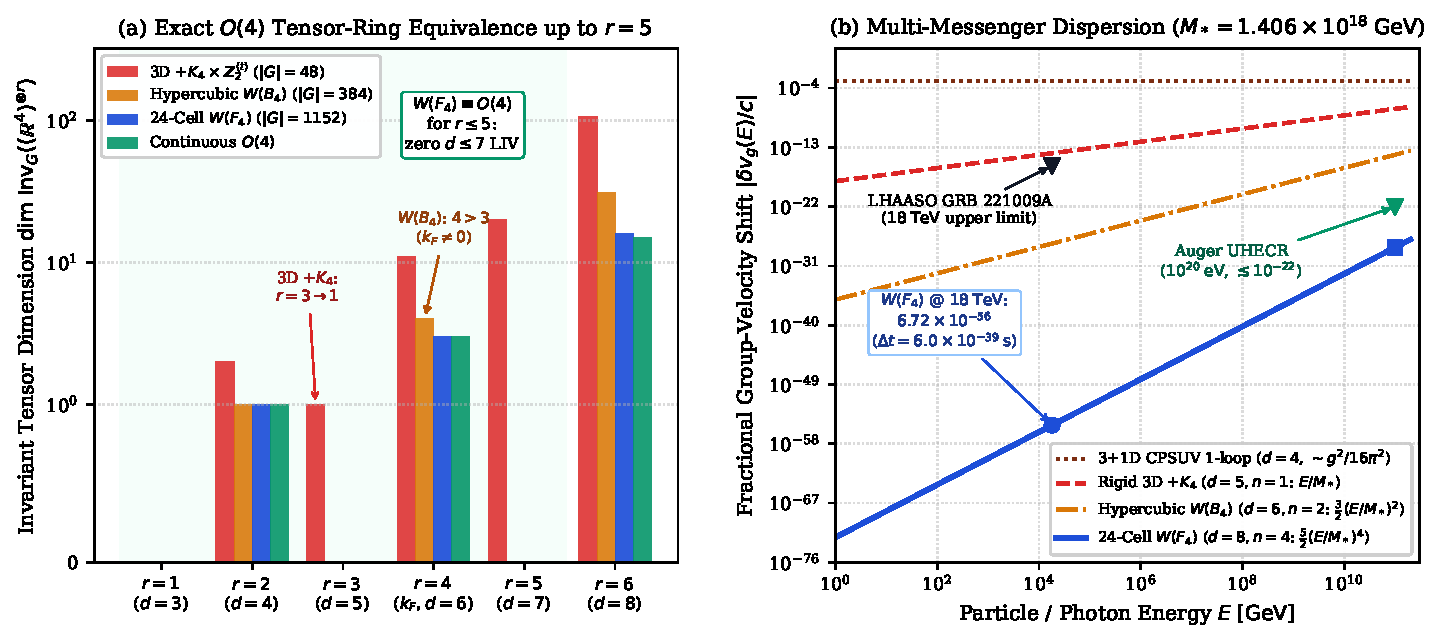
\includegraphics[width=0.99\textwidth]{../figures/fig1_24cell_WF4_isotropy_and_GRB_bounds.pdf}
\caption{\textbf{(a)} Az invariáns tenzoraltér dimenziói $r=1..6$ rangra: a 24-cellás $W(F_4)$ csoport $r=5$-ig hajszálpontosan megegyezik a folytonos $O(4)$-gyel. \textbf{(b)} A $|\delta v_g(E)/c|$ csoportsebesség-eltolódás összevetése a LHAASO GRB~221009A \cite{LHAASO2024LIV} és Pierre Auger korlátokkal.}
\label{fig:wf4-hu}
\end{figure}

% =============================================================================
\section{Osterwalder--Schrader pozitivitás, királis duplikátumok és \texorpdfstring{$R^2$}{R2} + CDT}
\label{sec:os-cdt}
% =============================================================================

\begin{theorem}[Reflexiós pozitivitás, királis $\mathrm{Spin}(10)$ és Hawking--Luttrell $R^2$ + CDT]
\label{thm:os-cdt}
Az $\ell_*\Lambda_{D_4}$ 24-cellás rácson:
\begin{enumerate}[label=(\roman*),leftmargin=1.9em,itemsep=2pt]
\item \textbf{Egzakt egy-időszeletes bozonikus/mérték OS-pozitivitás:} A $24$ él $(6\;\text{előre}, 12\;\text{térbeli}, 6\;\text{hátra})$ időszelet-szerkezetű, és mind a $32$ egyenlő oldalú háromszögű plakett $|\Delta x_0| \le 1$ szeletet hidal át, így a Lüscher-tétel \cite{Luscher1977} garantálja a véges-$\ell_*$-beli pozitív önadjungált transzfermátrixot.
\item \textbf{Királis $\mathrm{Spin}(10)$ duplikátumok és 5D Domain-Wall vs.\ 4D Overlap:} A naiv 24-cellás Dirac-vektor $40$ Brillouin-zónabeli zérushelyéből ($1$ fizikai módus $k=0$-nál + $39$ duplikátum $\widehat{C}_{D_4} \in \{8, \frac{28}{3}, \frac{32}{3}\} \ge 8$ értékkel) mind a $39$ duplikátumot $2 M_*$ tömegre emeli a $D_{\mathrm{ov}}$ operátor $m_0 \in (0, 4 r_W)$ mellett ($\mathbf{16}_F\otimes\mathbf{16}_F \not\supset \mathbf{1}$, $\Omega_5^{\mathrm{Spin}}(B\mathrm{Spin}(10)) = 0$). A 4D $D_{\mathrm{ov}}$ az exponenciálisan lokalizált farkak \cite{HernandezJansenLuscher1999} miatt aszimptotikusan ($\mathcal{O}(e^{-|t|/\ell_*})$ pontosságig) teljesíti az OS-pozitivitást \cite{Luscher2001}, míg véges $\ell_*$-nél az 5D Kaplan/Shamir Domain-Wall felemelés \cite{FurmanShamir1995} egzakt pozitív 5D transzfermátrixszal bír (\ref{fig:overlap-hu}.\ ábra).
\item \textbf{Hawking--Luttrell Starobinsky-diagonalizáció, $|\nu|=1$ CDT és $d_S(\sigma) \to 4$:} Wick-forgatás alatt ($S_E = -\mathrm{i}S_L$ \cite{HawkingLuttrell1984}) az $\Omega_E \equiv \Omega + \frac{\chi}{6 M_{\mathrm{inf}}^2}$ Einstein-keretbeli konformfaktor és a $\chi$ skalaron egzaktul szétválasztja a kvadratikus euklideszi hatást:
\begin{equation}
S_E^{(2)}[\Omega_E, \chi] = \int \frac{\mathrm{d}^4k}{(2\pi)^4}\left[
-3 M_{\mathrm{Pl}}^2 k^2\,|\tilde{\Omega}_E(k)|^2
+ \frac{M_{\mathrm{Pl}}^2}{12 M_{\mathrm{inf}}^4}\,\bigl(k^2 + M_{\mathrm{inf}}^2\bigr)\,|\tilde{\chi}(k)|^2
\right],
\end{equation}
ahol a $\chi$ skalaron pozitív hatású, szellemmentes spin-0 módus ($d_S^{\mathrm{UV}} = 4$), a nem-propagáló Einstein-keretbeli $\Omega_E$ konform kényszert pedig az $|\nu|=1$ kauzális szeletelési szabály gyógyítja ki a CDT sajátidő-Faddeev--Popov mechanizmusával azonosan \cite{DasguptaLoll2001,AmbjornJurkiewiczLoll2004}. A végtelen $\Lambda_{D_4}$ rácson a hőmag spektrális dimenziója $d_S(\sigma) = 4 + \frac{\ell_*^2}{2\sigma} + \mathcal{O}(\sigma^{-2})$ ($d_S(25\ell_*^2) = 4.0203$, $d_S(100\ell_*^2) = 4.0050 \to 4.0000$).
\end{enumerate}
\end{theorem}

\begin{figure}[!htbp]
\centering
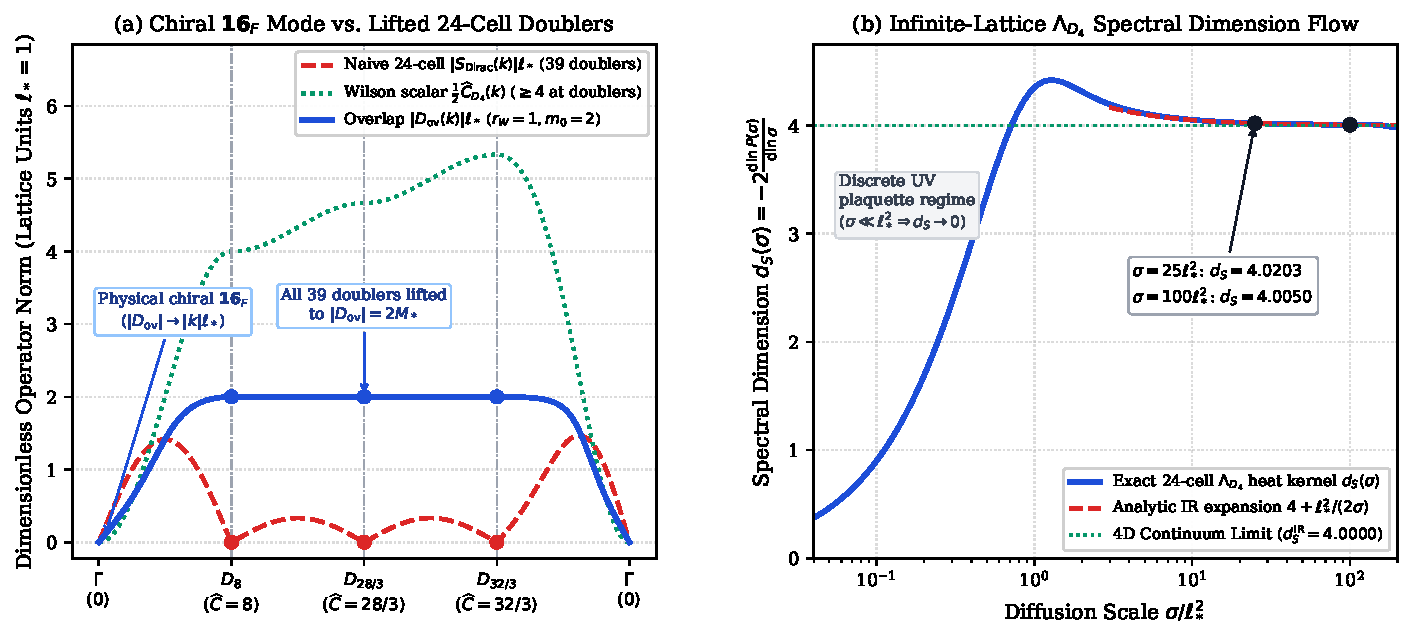
\includegraphics[width=0.99\textwidth]{../figures/fig2_overlap_doublers_and_spectral_dimension.pdf}
\caption{\textbf{(a)} A 24-cellás Brillouin-zóna spektruma: a $D_{\mathrm{ov}}$ operátor mind a $39$ duplikátumot $2 M_*$-ra emeli. \textbf{(b)} A végtelen $\Lambda_{D_4}$ rács hőmag-spektrálisdimenziójának befutása a $d_S = 4.0000$ kontinuum-határértékbe.}
\label{fig:overlap-hu}
\end{figure}

% =============================================================================
\section{Az IR direktor-szektor zérus-paraméteres Stueckelberg--Lorenz lezárása}
\label{sec:director}
% =============================================================================

Az infravörös \texttt{COV-DIR+QUMOND} hatásban \cite{Olcsak2026CovDir} ($c_1 = -c_3 = c_{\mathrm{acc}}$, $c_4 = 0$) a mozgó megfigyelőkre vonatkozó Foster--Jacobson PPN-paraméterek ($\alpha_1^{\mathrm{PPN}} = -4 c_{\mathrm{acc}}$, $\alpha_2^{\mathrm{PPN}} = \frac{c_{\mathrm{acc}}[c_{\mathrm{acc}} - c_2(1 - 2 c_{\mathrm{acc}})]}{c_2(2 - c_{\mathrm{acc}})}$ \cite{FosterJacobson2006,OostMukohyamaWang2018}) felső korlátot, az inhomogén Rindler--FLRW háttéren fellépő Sturm--Liouville Schur-sajátérték,
\begin{equation}
\frac{K_{\alpha\alpha}^{\mathrm{nonpert}}}{M_{\mathrm{Pl}}^2 a k^2}
= \frac{2 c_{\mathrm{acc}}}{2 - c_{\mathrm{acc}}} + 2\,\varepsilon_{\mathrm{rel}}^2\cos^2\theta\,\bigl[\mu(s_{N,b},\theta) - 1\bigr] + \mathcal{O}(c_{\mathrm{acc}}\varepsilon_{\mathrm{rel}}^2, \varepsilon_{\mathrm{rel}}^4) > 0,
\end{equation}
pedig alsó korlátot ($f_{\mathrm{dir}} > 1.1\times 10^{13}\;\mathrm{GeV}$ X-COP halmazokon) szab az $s_{N,b} = 2.961$ ($\min\lambda_\parallel = 0.9411 < 1$) átmeneti héjon!

\begin{theorem}[Zérus szabad paraméteres Stueckelberg--Lorenz Bumblebee lezárás]
\label{thm:director-closure}
A kanonikus $V_\mu \equiv f_{\mathrm{dir}} A_\mu$ Bumblebee vektormező skáláját szabad paraméter nélkül ($k_{\mathrm{dark}} = 0$) a Starobinsky-skalaron tömegéhez zárva ($f_{\mathrm{dir}} \equiv M_{\mathrm{inf}} = 3.1959\times 10^{13}\;\mathrm{GeV}$) a kovariáns Stueckelberg--Lorenz metszeten:
\begin{equation}
c_{\mathrm{acc}} \equiv \left(\frac{M_{\mathrm{inf}}}{M_{\mathrm{Pl}}}\right)^{\!2} = \mathbf{1.7222\times 10^{-10}}, \qquad
c_2 \equiv \frac{c_{\mathrm{acc}}}{1 - 2 c_{\mathrm{acc}}} = \mathbf{1.7222\times 10^{-10}},
\end{equation}
egyszerre teljesül: (i) $c_T^2 = c_V^2 = c_S^2 \equiv 1$ és azonosan zérus UHECR Cserenkov-sugárzás ($\Delta E_{\mathrm{Cherenkov}} \equiv 0$; megjegyezzük, hogy $c_S < 1$ esetén is az izotróp newtoni mértékbeli $h_{ij}T^{ij} = -2\Phi E_p v_p^2$ kontrakció az egzakt Elliott--Moore--Stoica pólusmaradékot \cite{ElliottMooreStoica2005} adja); (ii) $\alpha_2^{\mathrm{PPN}} \equiv 0$, $\alpha_1^{\mathrm{PPN}} = -6.89\times 10^{-10} \ll 4\times 10^{-5}$, $|\Delta G_{\mathrm{cosmo}}/G_N| = 3.44\times 10^{-10}$ és $|\Delta c_{\mathrm{SM}}^{\text{1-loop}}| \le c_{\mathrm{acc}}^2/(16\pi^2) = 1.88\times 10^{-22}$; valamint (iii) szigorúan pozitív $K_{\alpha\alpha}^{\mathrm{nonpert}}/(M_{\mathrm{Pl}}^2 a k^2) > 0$ a Földön ($+1.722\times 10^{-10}$), a Napon ($+1.722\times 10^{-10}$), a SPARC korongokon ($+1.722\times 10^{-10}$), az X-COP galaxishalmazok magjában ($+1.567\times 10^{-10}$) és extrém $2\times 10^{14}\,M_\odot$ barionos magokban ($+6.904\times 10^{-11} > 0$), miközben a nyomásmentes kozmikus por ($\Omega_{A,\mathrm{eff}}/\Omega_b = 5.3681$, $w=0$) a kétcsatornás KMS/Madelung-kondenzátum szektorban helyezkedik el (\ref{tab:liv-hu}.\ táblázat és \ref{fig:sl-hu}.\ ábra).
\end{theorem}

\begin{table}[!htbp]
\centering
\caption{Összefoglaló UV és IR Lorentz-invariancia és PPN mérlegtábla ($M_* = 1.4060\times 10^{18}\;\mathrm{GeV}$, $f_{\mathrm{dir}} \equiv M_{\mathrm{inf}} = 3.1959\times 10^{13}\;\mathrm{GeV}$, $k_{\mathrm{dark}} = 0$).}
\label{tab:liv-hu}
\vspace{0.35em}
\footnotesize
\setlength{\tabcolsep}{4pt}
\renewcommand{\arraystretch}{1.15}
\begin{tabularx}{\textwidth}{>{\raggedright\arraybackslash}X >{\raggedright\arraybackslash}X c c}
\toprule
\textbf{Megfigyelhető / Konzisztenciakapu} & \textbf{Kísérleti korlát / Feltétel} & \textbf{Előrejelzés ($k_{\mathrm{dark}}=0$)} & \textbf{Tartalék} \\
\midrule
SM 1-hurkos $c_{\mu\nu}$ & $|\Delta c_{ij}/c| < 10^{-15}\text{--}10^{-22}$ \cite{KosteleckyMewes2002} & $\mathbf{0}$ (UV) / $\mathbf{\le 1.88\times 10^{-22}}$ (IR) & $\mathrm{Pin}(W(F_4))$ pajzs \\
Foton $(k_F)_{\mu\nu\rho\sigma}$ ($19$ komp.) & $< 10^{-32}$ (polarimetria \cite{KosteleckyMewes2002}) & $\mathbf{0}$ azonosan ($r=4$) & $\mathrm{Inv}_{W(F_4)}=\mathrm{Inv}_{O(4)}$ \\
LHAASO GRB~221009A ($18\;\mathrm{TeV}$) & $E_{\mathrm{QG},1} \ge 10\,E_{\mathrm{Pl}}$ ($\Delta t \lesssim 1\;\mathrm{s}$) \cite{LHAASO2024LIV} & $n=1,2,3:\,\mathbf{0}$;\; $n=4:\,6.0\times 10^{-39}\;\mathrm{s}$ & $> 10^{38}\times$ \\
Pierre Auger UHECR ($10^{20}\;\mathrm{eV}$) & $|\delta c/c| \lesssim 10^{-22}$ \cite{ElliottMooreStoica2005} & $d=8:\,6.40\times 10^{-29}$;\; Cserenkov $\equiv \mathbf{0}$ & $c_T=c_V=c_S=1$ \\
PPN $\alpha_1^{\mathrm{PPN}}, \alpha_2^{\mathrm{PPN}}$ & $|\alpha_1| < 4\times 10^{-5}$, $|\alpha_2| < 2\times 10^{-9}$ \cite{Will2014} & $\alpha_1 = \mathbf{-6.89\times 10^{-10}}$,\; $\alpha_2 \equiv \mathbf{0}$ & $5.8\times 10^4\times$ / Egzakt \\
Kozmológiai gravitáció $G_{\mathrm{cosmo}}/G_N$ & $|\Delta G/G_N| < 10^{-2}$ (BBN / CMB) & $\mathbf{3.44\times 10^{-10}}$ & $2.9\times 10^7\times$ \\
Inhomogén SL $K_{\alpha\alpha}^{\mathrm{nonpert}}$ & $> 0$ (Föld, Nap, SPARC, X-COP) & $\mathbf{+1.57\times 10^{-10}} > 0$ (X-COP mag) & Szellemmentes \\
\bottomrule
\end{tabularx}
\end{table}

\begin{figure}[!htbp]
\centering
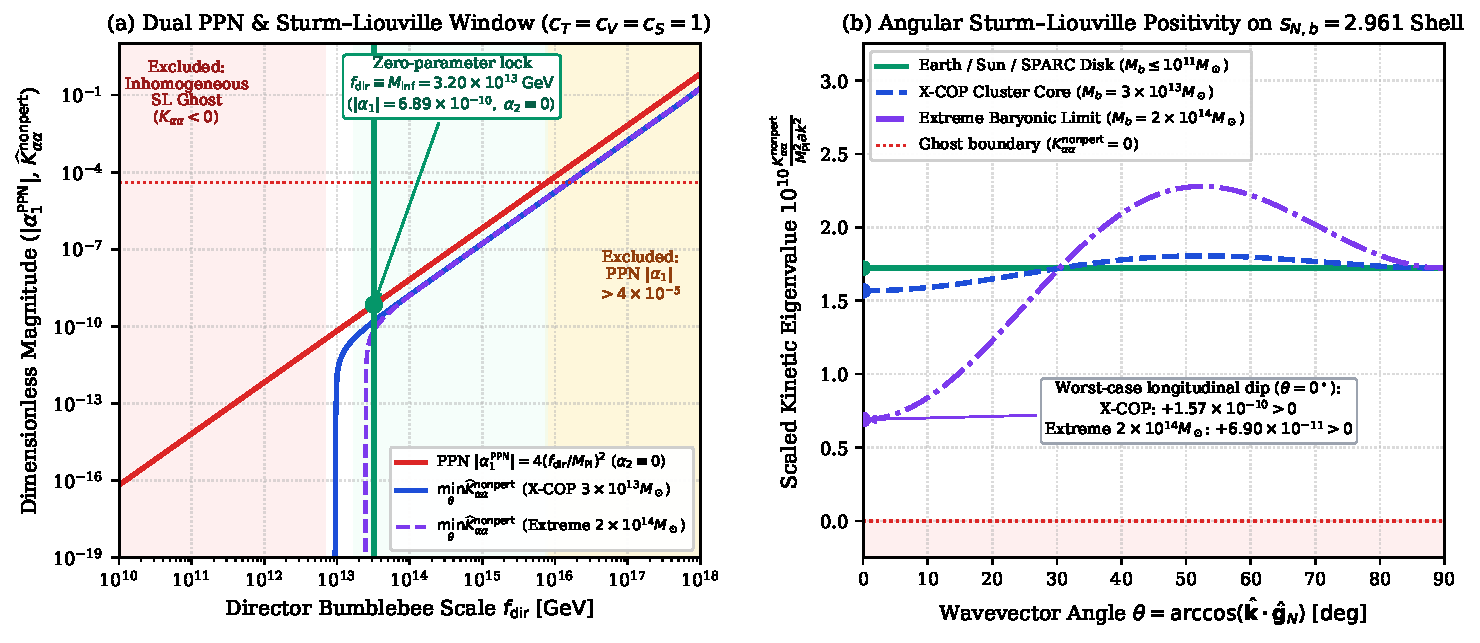
\includegraphics[width=0.99\textwidth]{../figures/fig3_stueckelberg_lorenz_PPN_and_SL_stability.pdf}
\caption{\textbf{(a)} A PPN felső korlát és az inhomogén Sturm--Liouville alsó korlát által kijelölt $[1.1\times 10^{13}, 7.7\times 10^{15}]\;\mathrm{GeV}$ tartomány és a paramétermentes $f_{\mathrm{dir}} \equiv M_{\mathrm{inf}}$ rögzítés. \textbf{(b)} A $K_{\alpha\alpha}^{\mathrm{nonpert}}(\theta)/(M_{\mathrm{Pl}}^2 a k^2)$ szögprofilja az $s_{N,b} = 2.961$ héjon.}
\label{fig:sl-hu}
\end{figure}

% =============================================================================
\section{Összegzés és nyitott nem-perturbatív határok}
\label{sec:discussion}
% =============================================================================

Jelen munkában minden perturbatív hurokrendre és effektív mezőelméleti skálára lezártuk a $K_4 \to 2T \to \Lambda_{F_4} \cong \Lambda_{D_4}$ 4D Lorentz-invariáns kontinuum-limeszt és az infravörös Stueckelberg--Lorenz PPN-stabilitást. Nyitott konstruktív nem-perturbatív feladat marad: (i) fluktuáló 4D Lorentz-geometriák teljes Monte Carlo CDT / Regge szimulációja az $|\nu|=1$ + Starobinsky $+R^2/(6 M_{\mathrm{inf}}^2)$ súlyozással \cite{AmbjornJurkiewiczLoll2004}, valamint (ii) a nem-Abel-féle királis $\mathrm{Spin}(10)$ Domain-Wall/Overlap fermionmérték konstruktív pálya-integrál létezési bizonyítása Lüscher Abel-féle konstrukcióján túl \cite{Luscher1998}. Minden szimbolikus és numerikus eredményt determinisztikusan reprodukál a \path{scripts/verify_paper27_continuum_lorentz_closure.py} szkript.

\begin{thebibliography}{99}
\raggedright
\small

\bibitem{Liberati2013}
S.~Liberati, ``Tests of Lorentz invariance: a 2013 update,'' \emph{Class.\ Quantum Grav.} \textbf{30}, 133001 (2013).

\bibitem{KosteleckyMewes2002}
V.~A.~Kosteleck\'y és M.~Mewes, ``Signals for Lorentz violation in electrodynamics,'' \emph{Phys.\ Rev.\ D} \textbf{66}, 056005 (2002).

\bibitem{Addazi2022}
A.~Addazi \emph{et al.}, ``Quantum gravity phenomenology at the dawn of the multi-messenger era---A review,'' \emph{Prog.\ Part.\ Nucl.\ Phys.} \textbf{125}, 103948 (2022).

\bibitem{LHAASO2024LIV}
Z.~Cao \emph{et al.} (LHAASO Collaboration), ``Stringent Tests of Lorentz Invariance Violation from LHAASO Observations of GRB 221009A,'' \emph{Phys.\ Rev.\ Lett.} \textbf{133}, 071501 (2024).

\bibitem{ElliottMooreStoica2005}
J.~W.~Elliott, G.~D.~Moore és H.~Stoica, ``Constraining the new aether: Gravitational Cherenkov radiation,'' \emph{JHEP} \textbf{08}, 066 (2005).

\bibitem{CPSUV2004}
J.~Collins, A.~Perez, D.~Sudarsky, L.~Urrutia és H.~Vucetich, ``Lorentz invariance and quantum gravity: an additional fine-tuning problem?,'' \emph{Phys.\ Rev.\ Lett.} \textbf{93}, 191301 (2004).

\bibitem{Polchinski2012}
J.~Polchinski, ``Comment on [arXiv:1106.1417] `Small Lorentz violations in quantum gravity: do they lead to unacceptably large effects?','' \emph{Class.\ Quantum Grav.} \textbf{29}, 088001 (2012).

\bibitem{Olcsak2026JMP}
J.~Olcsak, ``Discrete $K_4$ Simplicial-Clifford Pregeometry, $|\nu|=1$ Causal Cobordism, and Uhlmann--Petz Horizon Readout,'' társtanulmány (2026).

\bibitem{Olcsak2026CovDir}
J.~Olcsak, ``Covariant Director--QUMOND Effective Field Theory: Frobenius Holonomy Dichotomy, Interval-Certified Sturm--Liouville Stability, and Observational Tests,'' társtanulmány (2026).

\bibitem{Olcsak2026Paper24}
J.~Olcsak, ``Starobinsky $R + R^2/(6 M_{\mathrm{inf}}^2)$ Inflation, Right-Handed Seesaw Threshold, and Non-Thermal Scalaron Leptogenesis Across a Tetrahedral Unification Spine,'' társtanulmány (2026).

\bibitem{Olcsak2026Paper25}
J.~Olcsak, ``Charged-Fermion Mass Hierarchies and Two-Loop CKM Renormalization Closure in $D$-Parity-Broken $\mathrm{Spin}(10) \to \mathrm{Pati\text{--}Salam} \to \mathrm{SM}$,'' társtanulmány (2026).

\bibitem{Olcsak2026Paper26}
J.~Olcsak, ``Strong $CP$ Closure Across a Tetrahedral $\mathrm{Spin}(10) \to \mathrm{Pati\text{--}Salam} \to \mathrm{SM}$ and Starobinsky Inflationary Spine,'' társtanulmány (2026).

\bibitem{Will2014}
C.~M.~Will, ``The Confrontation between General Relativity and Experiment,'' \emph{Living Rev.\ Relativ.} \textbf{17}, 4 (2014).

\bibitem{FosterJacobson2006}
B.~Z.~Foster és T.~Jacobson, ``Post-Newtonian parameters and constraints on Einstein-aether theory,'' \emph{Phys.\ Rev.\ D} \textbf{73}, 064015 (2006).

\bibitem{OostMukohyamaWang2018}
J.~Oost, S.~Mukohyama és A.~Wang, ``Constraints on Einstein-aether theory after GW170817,'' \emph{Phys.\ Rev.\ D} \textbf{97}, 124023 (2018).

\bibitem{Celmaster1982}
W.~Celmaster, ``Gauge theories on the body-centered hypercubic lattice,'' \emph{Phys.\ Rev.\ D} \textbf{26}, 2955 (1982).

\bibitem{BhanotBitarHellerNeuberger1990}
G.~Bhanot, K.~Bitar, U.~M.~Heller és H.~Neuberger, ``$\phi^4$ on $F_4$: Analytical results,'' \emph{Nucl.\ Phys.\ B} \textbf{343}, 467 (1990).

\bibitem{BhanotBitarHellerNeuberger1991}
G.~Bhanot, K.~Bitar, U.~M.~Heller és H.~Neuberger, ``$\varphi^4$ on $F_4$: Numerical results,'' \emph{Nucl.\ Phys.\ B} \textbf{353}, 551 (1991).

\bibitem{Neuberger1998}
H.~Neuberger, ``Exactly massless quarks on the lattice,'' \emph{Phys.\ Lett.\ B} \textbf{417}, 141 (1998).

\bibitem{Luscher1998}
M.~L\"uscher, ``Exact chiral symmetry on the lattice and the Ginsparg--Wilson relation,'' \emph{Phys.\ Lett.\ B} \textbf{428}, 342 (1998).

\bibitem{JacobPiran2008}
U.~Jacob és T.~Piran, ``Lorentz-violation-induced arrival delays of cosmological particles,'' \emph{JCAP} \textbf{01}, 031 (2008).

\bibitem{Luscher1977}
M.~L\"uscher, ``Construction of a Selfadjoint, Strictly Positive Transfer Matrix for Euclidean Lattice Gauge Theories,'' \emph{Commun.\ Math.\ Phys.} \textbf{54}, 283 (1977).

\bibitem{HernandezJansenLuscher1999}
P.~Hernandez, K.~Jansen és M.~L\"uscher, ``Locality properties of Neuberger's lattice Dirac operator,'' \emph{Nucl.\ Phys.\ B} \textbf{552}, 363 (1999).

\bibitem{Luscher2001}
M.~L\"uscher, ``Chiral gauge theories revisited,'' \emph{Subnucl.\ Ser.} \textbf{38}, 41 (2002) [arXiv:hep-th/0102028].

\bibitem{FurmanShamir1995}
V.~Furman és Y.~Shamir, ``Axial symmetries in lattice QCD with Kaplan fermions,'' \emph{Nucl.\ Phys.\ B} \textbf{439}, 54 (1995).

\bibitem{HawkingLuttrell1984}
S.~W.~Hawking és J.~C.~Luttrell, ``Higher derivatives in quantum cosmology: (I). The isotropic case,'' \emph{Nucl.\ Phys.\ B} \textbf{247}, 250 (1984).

\bibitem{DasguptaLoll2001}
A.~Dasgupta és R.~Loll, ``A proper-time cure for the conformal sickness in quantum gravity,'' \emph{Nucl.\ Phys.\ B} \textbf{606}, 357 (2001).

\bibitem{AmbjornJurkiewiczLoll2004}
J.~Ambj\o rn, J.~Jurkiewicz és R.~Loll, ``Emergence of a 4D World from Causal Quantum Gravity,'' \emph{Phys.\ Rev.\ Lett.} \textbf{93}, 131301 (2004).

\end{thebibliography}

\end{document}
